\documentclass[12pt]{article}
\usepackage{fullpage,epic,eepic,epsfig,makeidx,color,graphicx,moreverb,boxedminipage,version}
\sloppy

\excludeversion{tobedone}


\newcommand{\C}{\texttt{C}}
\newcommand{\gpl}{Gnu Public License}
\newcommand{\pip}{PiP}
\newcommand{\lpsolve}{LP-Solve}

\newcommand{\sitemmalfa}
{\texttt{{http://www.irisa.fr/cosi/ALPHA}{http://www.irisa.fr/api/ALPHA}}}
\newcommand{\emailmmalfa}{\texttt{alpha@irisa.fr}}

\newcommand{\Alpha}{{\sc Alpha}}
\newcommand{\AlpHard}{{\sc AlpHard}}
\newcommand{\MMA}{{\sc MMAlpha}}
\newcommand{\api}{{\sc api}}
\newcommand{\irisa}{ Irisa}
\newcommand{\vlsi}{{\sc vlsi}}
\newcommand{\vhdl}{{\sc vhdl}}
\newcommand{\alfa}{\Alpha}
\newcommand{\mmalfa}{\MMA}
\newcommand{\MMAlfa}{\MMA}
\newcommand{\mmalpha}{\MMA}
\newcommand{\mma}{{Mathematica}}
\newcommand{\polylib}{{\sc polylib}}
\newcommand{\Opt}[1]{{\rm\sl [} #1 {\rm\sl ]}}
\newcommand{\Group}[1]{{\rm\sl (} #1 {\rm\sl )}}
\newcommand{\Alt}{$\mid$}
\newcommand{\Program}{{\sl Program\ }}
\newcommand{\PDecl}{{\sl PDecl\ }}
\newcommand{\PointwiseDecl}{{\sl PointwiseDecl\ }}
\newcommand{\SystemDecl}{{\sl SystemDecl\ }}
\newcommand{\Name}{{\sl Name\ }}
\newcommand{\ScalarInDeclList}{{\sl ScalarInDeclList\ }}
\newcommand{\ScalarOutDecl}{{\sl ScalarOutDecl\ }}
\newcommand{\ScalarLocDeclList}{{\sl ScalarLocDeclList\ }}
\newcommand{\ScalarVarDecl}{{\sl ScalarVarDecl\ }}
\newcommand{\ScalarDeclList}{{\sl ScalarDeclList\ }}
\newcommand{\InputDeclList}{{\sl InputDeclList\ }}
\newcommand{\OutputDeclList}{{\sl OutputDeclList\ }}
\newcommand{\LocalDeclList}{{\sl LocalDeclList\ }}
\newcommand{\VarDeclList}{{\sl VarDeclList\ }}
\newcommand{\EquationBlock}{{\sl Equationblock\ }}
\newcommand{\ParamDecl}{{\sl ParamDecl\ }}
\newcommand{\VarDeclaration}{{\sl VarDeclaration\ }}
\newcommand{\Domain}{{\sl Domain\ }}
\newcommand{\IdentifierList}{{\sl IdentifierList\ }}
\newcommand{\Identifier}{{\sl Identifier\ }}
\newcommand{\ScalarType}{{\sl ScalarType\ }}
\newcommand{\IndexList}{{\sl IndexList\ }}
\newcommand{\ConstraintList}{{\sl ConstraintList\ }}
\newcommand{\AffineFunction}{{\sl AffineFunction\ }}
\newcommand{\Constraint}{{\sl Constraint\ }}
\newcommand{\IncreasingSeq}{{\sl IncreasingSeq\ }}
\newcommand{\DecreasingSeq}{{\sl DecreasingSeq\ }}
\newcommand{\EqualitySeq}{{\sl EqualitySeq\ }}
\newcommand{\IndexExpList}{{\sl IndexExpList\ }}
\newcommand{\EquationList}{{\sl EquationList\ }}
\newcommand{\Equation}{{\sl Equation\ }}
\newcommand{\ParamAssignation}{{\sl ParamAssignation\ }}
\newcommand{\InputList}{{\sl InputList\ }}
\newcommand{\ExtParamAssgn}{{\sl ExtParamAssgn\ }}
\newcommand{\ExtensionDomain}{{\sl ExtensionDomain\ }}
\newcommand{\ExpressionList}{{\sl ExpressionList\ }}
\newcommand{\Expression}{{\sl Expression\ }}
\newcommand{\Constant}{{\sl Constant\ }}
\newcommand{\IntegerConstant}{{\sl IntegerConstant\ }}
\newcommand{\RealConstant}{{\sl RealConstant\ }}
\newcommand{\BooleanConstant}{{\sl BooleanConstant\ }}
\newcommand{\BinaryOp}{{\sl BinaryOp\ }}
\newcommand{\CommutativeOp}{{\sl CommutativeOp\ }}
\newcommand{\RelativeOp}{{\sl RelativeOp\ }}
\newcommand{\UnaryOp}{{\sl UnaryOp\ }}
\newcommand{\IndexExpression}{{\sl IndexExpression\ }}
\newcommand{\IndexTerm}{{\sl IndexTerm\ }}
\newcommand{\Number}{{\sl Number\ }}
\newcommand{\Digit}{{\sl Digit\ }}
\newcommand{\Letter}{{\sl Letter\ }}
%\newcommand{\}{{\sl \ }}

\newcommand {\setn}   {\hbox{\it I\hskip -2pt N}}     % ensemble N
\newcommand {\setz}   {\hbox{\it Z\hskip -4pt Z}}     %ensemble Z
\newcommand {\setq}   {\hbox{\it Q\hskip -6pt {\it l}\hskip 4pt}}     % ensemble Q

\newcounter{Nex}

\newtheorem{ex}{Exemple}[section]
%\newenvironment{ex}
%{\vspace{0.5cm} \refstepcounter{Nex} {\bf Example ${\theNex}$:}
%\begin{quotation}}
%{\end{quotation}}

\makeindex

\begin{document}

\title{Getting started with \Alpha{}}
\author{Api, then Cosi, then R2D2 and Compsys\thanks{
Api, Cosi and R2D2 are the names of the 
research groups that successively hosted
research related on \alfa{} and \mmalpha{} at Irisa, Rennes, France. 
From 2001, Compsys in ENS Lyon also participated in 
the development of \mmalpha{}. Recently, Tanguy Risset moved to \textsc{Insa} de Lyon.}
\\Revision of \today{}}
\date{June 2004}
\maketitle

\begin{abstract}
This document is an introduction to the \alfa{} language
and to its use for regular program description, transformation, 
evaluation, and hardware implementation in the \mmalfa{} 
software. The \alfa{} syntax is presented by means of examples. 
Basic manipulations of \alfa{} programs are first shown. 
Then hardware generation and 
several advanced 
transformations -- pipelining, change of basis, substitution, 
normalization, and 
scheduling, -- are introduced and illustrated. 
Finally, the use of \alfa{} subsystems and the \AlpHard{}
hardware description language are presented.
\end{abstract}

\section{Introduction}
\label{intro}
This document\footnote{The source of this document is in:\\
\texttt{\$MMALPHA/doc/Quickstart/AlphaStart.tex}\\
and this file is in\\
\texttt{\$MMALPHA/doc/QuickStart/AlphaStart.pdf}\\
} should be read by all \alfa{} beginners.
It briefly presents the main features of the \alfa{} language and
the basic transformations of \alfa{} programs which are 
available in the \mmalfa{} environment.

\mmalfa{} is a free software, available under the 
\gpl{}. It can be downloaded from 
the site: 

\sitemmalfa{}. 

To be run, it requires
\mma{} version 3.0 or later.

If you have any problem while reading this document or while 
trying the
\mmalfa{} software, please send an e-mail to \emailmmalfa{}

\subsection*{What is \Alpha?}
\label{Whatis}
\nocite{Alpha97a,BQRR,Ris21,DupontQuRi95,DuRiRo97,QuRaRi96a,QuRaRi97a}
{\Alpha} is a functional data parallel 
language invented at 
{\irisa} in Rennes (France). 
The first definition of \alfa{} was proposed by Mauras~\cite{Mauras89} 
in 1989. The original motivation was to provide 
a language for expressing algorithms in an extended version of 
the formalism of recurrence equations
proposed by Karp, Miller and Winograd~\cite{KaMiWi67}. 
Other basic references are~\cite{Moldovan82,Quinton84c,Rajopadhye86}.
The goal of \alfa{} is to provide
a high-level tool for the synthesis of parallel regular {\vlsi} architectures.

Although {\Alpha} stands for the language itself, it is often also
associated with the environment in which it is currently developed:
{\bf {\MMA}}. {\MMA} is an interface based on the \mma{}
software from which one can manipulate {\Alpha} programs.

\mmalfa{} is still under development at \irisa{} and at ENS Lyon (France).

\subsection*{What is {\Alpha} for?}
\label{whatfor}
{\Alpha} is a research tool for 
various computer science fields such as functional language semantics,
parallelization, code generation, optimization, polyhedral theory,
{\vlsi} synthesis, systolic arrays, etc.

One important long term goal of \alfa{} is to promote the use of high-level 
functional languages for the synthesis of (parallel) {\vlsi}
architectures. From the short term, Alpha can be useful
for:
\begin{itemize}
\item Providing a correct recurrence equation specification for a particular 
algorithm (see section~\ref{language} and \ref{basic}).
\item Simulating such a specification (see section~\ref{simulation}).\index{Simulation}
\item Transforming and simplifying a recurrence equation specification (see 
sections~\ref{basic} and~\ref{advanced}).
\item Computing on convex polyhedra 
(see also~\texttt{{http://www.irisa.fr/polylib}}).
\index{polylib@\polylib}
\item Scheduling programs and detecting parallelism 
(see section~\ref{schedule}).
\end{itemize}

If you are ready to invest a little more time on {\MMA}, you will 
probably be able to:
\begin{itemize}
\item Generate {\vhdl} from this description.
\item Provide a design path from the high-level functional specification of
an algorithm to the layout description of a {\vlsi} algorithm
which implements it.
\end{itemize}

The remaining of this document is organized as follows. Section~\ref{howwork}
presents the \mmalfa{} interface; section~\ref{install} explains
the installation procedure; in section~\ref{language}, the \alfa{}
language is briefly presented, while in section~\ref{basic}, 
basic operations on \alfa{} programs are described; hardware
generation is presented in section~\ref{hardware}; in section~\ref{advanced},
other transformations of \alfa{} programs are explained, and 
in section~\ref{structured}, we explain how structured \alfa{} programs
can be structured and transformed. Finally, section~\ref{andnow}
concludes and gives some additional references for further 
exploration of \MMAlfa{}.

\section{How does \mmalfa{}{} work?}
\label{howwork}
{\mmalfa{}} is written in C and in \mma{}, but a user should only see
it through its \mma{} interface.

\mma{} provides an interpreted language with
high-level built-in functions for symbolic computations: {\mmalfa{}}
uses these facilities for transforming {\Alpha} programs. 
\mma{}\index{Mathematica@\mma{}}
embeds
also a general-purpose programming language. 

The basic principle of the {\mmalfa{}} environment is the following one:
\mma{} sto\-res an internal representation of an {\Alpha} program
(called Abstract Syntax Tree or AST)\index{Abstract Syntax Tree}\index{AST}
and performs computations on this
internal representation via the user's commands or functions. These commands
can be for example: view an {\Alpha} program, check
its correctness, generate \C{} code to simulate it, generate
\vhdl{} code, etc. 
All these transformations are done on the AST which is stored
in a \mma{} variable named \texttt{\$result}.
\index{result@\texttt{\$result}}

Specific \C{} functions are used for two purposes: parse and unparse
\alfa{} programs or expressions, and perform computations on
polyhedra. All \C{} functions are called via \mma{}.
Most of them are available separately in the \polylib{}
\index{the polyhedral library@\polylib{}}
polyhedral library which constitutes the computationnal kernel of the
{\mmalfa{}} environment.

\section{Installing \mmalfa{}}
\label{install}
\index{Installation@Installing \mmalfa{}}
Before going on, you
should install the {\mmalfa{}} environment. 
The installation procedure is explained in
the \MMAlfa{} web site (\sitemmalfa{}).

The easiest way to use \mmalfa{} is to access it 
through its notebook interface. 
\index{notebook interface}
To do so, type \texttt{mathematica} under
\texttt{Unix}, or start \mma{}~3.0 in the Programs menu of 
Windows NT\footnote{Any \mma{} version later than 3.0 will work.}.
\footnote{One can also access 
the \mma{} kernel directly. Type \texttt{math} under
\texttt{Unix}, or start \mma{}~3.0~Kernel in the Programs menu of 
Windows NT. An alternative is to use the \mma{} 
kernel via \texttt{emacs}, but then the demonstration notebooks are
not accessible.}

Once \mmalfa{} is installed, open a new \mma{} notebook
and evaluate the command \texttt{start[]} in this notebook\footnote{Type the command, then press simultaneously the Shift and Enter keys.}.
\index{start@\texttt{start[]}}
This command opens a demonstration notebook which is part
of the \mmalfa{} distribution. 
Then open the cell named "Introduction Notebooks"\footnote{For 
the reader who is not yet familiar with \mma{}'s 
notebooks, notebooks are organized as a tree of cells. Each cell is
delimited by a brackets at its right. Selecting a cell (and all 
its subcells) is done by clicking once its bracket. 
To open a cell, double-click the bracket once the cell is selected.}, 
\index{Introduction notebooks}
and click on button "Getting started". This opens a notebook where all 
the examples of this document are shown.
\index{Getting-started notebook}

\section{The \alfa{} language}
\label{language}
In this section, we present the syntax of the \alfa{} language. 
\index{syntax of alpha@syntax of \alfa{}}
\subsection{{\Alpha} through examples}
\label{alphabyexamples}
We introduce here the basic
features of the language on the matrix-vector multiplication example
shown in Fig.~\ref{fig1}.

\begin{figure}[htbp]
\begin{verbatim}
system prodVect: {N | N>1}
  (a : {i,j|1 <= i,j <= N} of integer; 
   b : {i|1 <= i <= N} of integer)
returns (c : {i|1 <= i <= N} of  integer);
var 
  C :  {i,j|1 <= i <= N; 0<= j <=N} of  integer;
let
  C[i,j] = 
    case
      {|j=0} : 0[];
      {|j>=1} : C[i,j-1] + a[i,j] * b[j];
    esac;
  c[i]=C[i,N];
tel;   
\end{verbatim}
\caption{{\Alpha} program describing the matrix vector product}
\label{fig1}
\end{figure}


\subsection*{Systems, variables, domains and parameters}
An {\Alpha} program is a {\em system}. \alfa{} variables are generalized
arrays which can have any shape (not just rectangles).  The set of
indices of the array is called the {\em domain} of the variable.
\index{system}
\index{domain}
\index{variable}
Example~\ref{ex1} below shows the declaration of a variable {\tt a}
whose domain is the set of points $(i,j)$ in the triangle 
$\{0 \leq i \leq j;j \leq 10\}$.
\begin{ex}{~}
\begin{verbatim}
a : {i,j | 0<= i <= j; j <=10} of integer
\end{verbatim}
\label{ex1}
\end{ex} 
In the example of Fig.~\ref{fig1}, domains are indexed
by a parameter \texttt{N} which is declared, together with its
domain, right after the system name. The values of the parameters
can be constrained by any kind of 
affine constraints. In 
general, parameters allow generic descriptions of algorithms to 
be specified. 

\subsection*{Input, output and local variables}
An \alfa{} system has input and output variables. 
Here inputs are \texttt{a} and \texttt{b}, and output
is \texttt{c}.
It may have local
variables, such as \texttt{C} here. Local variables are
declared after the keyword \texttt{var}.
\index{input variable}
\index{local variable}
\index{output variable}

\subsection*{Equations and expressions}
Each variable is defined by a unique equation which
usually has the form of a recurrence equation. 
\index{expression}
\index{equation}

The {\tt case}
construct allows one to define different values in different parts of
the domain.
\index{case expression}\index{case expression@\texttt{case}}

\begin{ex}{~}
\begin{verbatim}
a[i,j] = 
  case
    {| j = 0 } : 0[];
    {| j > 0 } : a[i,j-1]+1[];
  esac;
\end{verbatim}
\label{ex2} 
\end{ex}

The {\Alpha} expression of example~\ref{ex2} defines the values of
\texttt{a[i,0]} to be zero\footnote{Syntactic note: constants are zero
dimensional arrays hence the empty brackets in \texttt{0[]}.}
and recursively defines {\tt a} at all other points in its
domain. This equation defines a variable {\tt a} such that {\tt
a[i,j]=j}. 

In Fig.~\ref{fig1}, variable \texttt{C} is also defined as
a recurrence equation, and its value at point $(i,j)$ 
is $\sum_{j=1}^{j=i} a_{i,j} \times b_{j}$.

\subsection{Array notation and standard notation}
The above equations use the so-called 
{\em array notation} of \alfa{}. 
\index{array notation}
\index{standard notation}
The
real syntax of {\Alpha} is sligthly less readable but more consistent
and logical from a semantic point of view. To illustrate this,
example~\ref{ex3} shows the same definition of {\tt a} in standard
notation.
\begin{ex}{~}
\begin{verbatim}
a = 
  case
    {i,j | j = 0 } : 0.(i,j -> );
    {i,j | j > 0 } : a.(i,j -> i,j-1) + 1.(i,j -> );
  esac;
\end{verbatim}
\label{ex3}
\end{ex}

\newcommand{\integer}{\texttt{integer}}
In such an expression, \texttt{a} denotes a variable, i.e., 
a function whose type is 
$$\integer{} \times \integer{} \rightarrow \integer{} \quad.$$
Expression \texttt{(i,j->i,j-1)} denotes
a dependence function\index{dependence function}, i.e., the affine function 
$$\integer{} \times \integer{} \rightarrow \integer{} \times \integer{}$$
which maps \texttt{(i,j)} to \texttt{(i,j-1)}. 
Expression \texttt{expr = a.(i,j->i,j-1)} denotes
the composition of \texttt{a} and the dependency function 
\texttt{(i,j -> i,j-1)}. 
In
other words, {\tt expr[i,j]} has the value {\tt a[i,j-1]} at each point
\texttt{(i,j)} such that \texttt{(i,j-1)} is in the domain of {\tt a}. 

Similarly {\tt expr2 = 0.(i,j->)} means that {\tt expr2[i,j]} has
value \texttt{0} for all \texttt{(i,j)}. This notation describes
the extension (or broadcasting) of the constant \texttt{0} to 
all integral points \texttt{(i,j)} of the space.\index{constant}

An expression such as \texttt{\{i,j | j > 0 \} : a.(i,j->i,j-1) + 1.(i,j->)}
represents the restriction of expression\index{restriction}
\texttt{a.(i,j->i,j-1) + 1.(i,j->)} to the 
domain \texttt{\{i,j | j > 0\}} (functions of \alfa{} are
partial).

Finally, \texttt{expr = case exp1; exp2; esac} denotes 
a case definition, where \texttt{exp1} and \texttt{exp2} are
expressions on disjoint domains.\index{case expression}

In summary, any \alfa{} expression is either a variable, 
the composition of a variable and of a dependence function, 
a restriction, or a case statement\footnote{There exists another
construct, the \texttt{use} statement, which allows calls
to subsystems to be written. This statement is explained in 
section~\ref{structured}.}.

Note that the order of the equations as well as the order of the
expressions in a case statement is meaningless
as \alfa{} is declarative:
interchanging the two branches of the case in
example~\ref{ex2} would define exactly the same value for {\tt a}.

The
evaluation order is implicit and there are tools for finding schedules
for a given program. As {\Alpha} is a functional language, the only
constraint that any evaluation order must follow is that data
dependencies between instances of 
variables must be respected. In example~\ref{ex2},
obviously {\tt a[i,j]} must be computed after {\tt a[i,j-1]}.

\subsection{More on the syntax of \alfa{}}
Section~\ref{sectstruct} describes structured \alfa{} programs.
More details on the syntax of \alfa{} can be found in
appendix~\ref{alpha1}. 
Note that \alfa{} is case sensitive, and that 
underscores are allowed in identifiers. Avoid using 
underscores, as you might get into trouble when trying to 
generate \vhdl{} for example.

\section{Basic operations on {\Alpha} programs}
\label{basic}

This section presents the first commands that you should learn in
order to deal with {\Alpha} programs. 

Write an {\Alpha}
program (such as the one of Fig.~\ref{fig1} for instance) using your
favourite text editor. 

Let us say you called this file \texttt{prodVect.alpha}.
The commands described in this section allow you to
{\bf load} your program in \mma{}, {\bf view} the program in
\mma{} (array notation or standard notation), {\bf save} the
program in another file, perform a {\bf static analysis} and {\bf simulate}
the program. 

All these examples are also available
in the \texttt{Getting started} notebook accessible by the 
\texttt{Master} notebook of \mmalfa{} (after starting
\mma{}, type the \mma{} command
{\tt start[]} in your notebook to  access the \texttt{Master} notebook of \mmalfa{}.)

If you are not familiar with \mma{}, the 
Introduction 
notebooks section of the
\texttt{Master} notebook
points towards a brief introduction to \mma{}.

\subsection{Loading and viewing an {\Alpha} program}
Once \mma{} has been started, commands can be send to 
the kernel through \texttt{Input} cells. 
\index{Directory@\texttt{Directory[]}}
The name of the working directory can be printed out
by typing:
\begin{verbatim}
Directory[]
\end{verbatim}

If you see that this directory is not the one where you have put 
{\tt prodVect.alpha}, change it by typing:
\begin{verbatim}
SetDirectory[ "pathname" ]
\end{verbatim}
\index{SetDirectory@\texttt{SetDirectory}}
where \texttt{pathname} is 
the directory that you want to become the current directory of 
\mmalpha{} (see the \mma{} Help or type \texttt{?Directory}).

You can now {\bf load} the {\Alpha} program into \mma{}
by typing:\\
\begin{verbatim}
load["prodVect.alpha"];
\end{verbatim}
\index{load@\texttt{load}}
\begin{small}
\begin{quotation}
Note that most often, it is useful to end 
\mmalfa{} commands with a semi-colon.
Indeed, \mmalfa{} commands are \mma{} functions, 
which return the AST of a transformed \alfa{} program.
If you forget the {\tt ;} symbol, 
\index{;@\texttt{;}}
\mma{} just displays the result of the function evaluation, 
which may sometimes take a few pages... 
\end{quotation}
\end{small}

As a side effect, the \texttt{load} command assigns the AST of
the parsed program to 
the global \mma{} variable {\tt \$result}\index{result@\texttt{\$result}}. 
In general, 
\texttt{\$result} contains the result of the most recent transformation.

\paragraph*{Troubleshooting}
Syntax errors in \alfa{} programs are sometimes difficult to understand. Here is 
a list of frequent errors.
\begin{itemize}
\item In domains, inequalities are separated by semicolons, not
colons. For example: \texttt{\{i | i<10 ; i> 20 \}}. Notice
that the domain \texttt{\{i,j | 1< i,j <20 \}}
represents the domain $\{i,j | 1 < i < 20 \wedge 
1 < j < 20 \}$, as the colon allows inequalities to 
be factorized.
\item Input variables are separated by semicolons.
\item All equations (even the last one) are ended by a semicolon.
\item All branches of a case (even the last one) are ended by a semicolon.
\item In the array notation, 
indexes of a right-hand side expression should appear in 
the right-hand side variable. For
example, \texttt{a[i,j] = b[k]} is wrong, as \texttt{k} is
not an index of \texttt{a}. Note that indexes represent 
positions, not absolute names. It is perfectly possible 
to use different index names in the declaration of a
variable, and in its definition, although this is a
bad practice...
\item Constants, such as \texttt{1[]} end up with brackets; boolean
constants are \texttt{true[]} and \texttt{false[]}.
\item Restrictions on branches of a case expression start with
\texttt{\{|}. 
\end{itemize}

\paragraph*{Bugs}
The \texttt{div} operator is available, but should be
replaced by a simple \texttt{/}. The \texttt{asave} function 
forgets to add a space after the \texttt{div} operator, so that
\texttt{a div 2[]} becomes \texttt{a div2[]}...

\subsection{Viewing {\Alpha} programs}
You can view the program that has been stored in {\tt \$result}\index{result@\texttt{\$result}} by 
evaluating:
\begin{verbatim}
ashow[]
\end{verbatim}
\index{ashow@\texttt{ashow}}
By default, \texttt{ashow} pretty prints the program contained 
in {\tt \$result}\index{result@\texttt{\$result}} in array notation, but more generally, \texttt{ashow[ var ]}
pretty prints the program contained in the \mma{} variable \texttt{var}.

To display a program in standard notation
use the
\texttt{show[]} command.
\index{show@\texttt{show}}
\subsection{On-line documentation and options}
\index{on-line documentation}
\index{options}
All \mma{} functions have an on-line documentation: 
\texttt{?ashow} gives the help on \texttt{ashow}. Commands
may also have options. Type \texttt{Options[ command ]} to list
the options of \texttt{command} together with their default value.
\index{on-line documentation}
\index{options}

The documentation of \MMAlfa{} is far from complete. 
Documentation notebooks are in directory 
\begin{verbatim}
$MMALPHA/doc/packages/
\end{verbatim}
and demos notebooks are available in 
\begin{verbatim}
$MMALPHA/demos/NOTEBOOKS/
\end{verbatim}
Documentation notebooks can be accessed
using the command \texttt{docLink[ "topic" ]}, and demos
can be open using \texttt{demoLink[ "demo" ]}: both commands
paste an active button in the current notebook. Try 
for example 
\begin{verbatim}
demoLink["Getting-started"]
\end{verbatim}

\subsection{Saving a program}
To save the {\Alpha} program in a file, use
the command {\tt asave} (or {\tt save} which saves in standard
notation). For instance: 
\begin{verbatim}
asave["myFile.alpha"]
\end{verbatim}
\index{asave@\texttt{asave}}
writes the program of Fig.~\ref{fig1} in file {\tt
myFile.alpha} in the current directory. 
This command is useful in order to save
the content of \texttt{\$result}\index{result@\texttt{\$result}} after some transformations. 

\subsection{Analyzing an {\Alpha} program}
\label{analyzing}
Now that you have loaded an {\Alpha} program, you can start working on
it. Your first action should always be to check it for so-called {\em static
errors} by using the {\tt analyze} command:
\begin{verbatim}
analyze[]
\end{verbatim}
\index{analyze@\texttt{analyze}}
Information about potential errors in the {\Alpha} program
is printed out. 

If the analysis is successful, the result is {\tt
True}. The static analyzer of \alfa{} does essentially two kinds
of verification: 
it checks the type of all expressions -- this is not a fantastic 
novelty -- but it also checks that variables are defined
in any point of their definition domain. This second kind of
verification is very powerful, and is much more original. 
\index{checking alpha programs@checking \alfa{} programs}

\paragraph*{Notes.}
\begin{itemize}
\item It is very important that your program passes successfully the 
\texttt{analyze} test. Indeed, some transformations assume that the program
is correct. 
\item Correcting the mistakes of an \alfa{} program may 
sometimes be difficult. Especially hard to fix are errors
involving values of the parameters. Do not hesitate to send 
a program to \emailmmalfa{} if you have some trouble: experts
will try to help you!
\item 
The \texttt{analyze} command allows structured systems to 
be checked by means of the \texttt{recurse} option. 
See \texttt{?recurse}.
\index{recurse@\texttt{recurse}}
\end{itemize}

\paragraph*{Troubleshooting}
If you use non conventional types, such as signed or 
unsigned short integer (denoted as \texttt{integer[S,5]} for
example), \texttt{analyze} is unable to check the type correctness
of expressions. Use the option \texttt{scalarTypeCheck -> False}
option to avoid error messages. 
\index{signed integers}
\index{unsigned integers}

\paragraph*{More information}
A notebook giving more details on the static analyzer can 
be accessed using \texttt{demoLink["Static"]}.
\index{demoLink@\texttt{demoLink}}

\subsection{Simulating a program}
\label{simulation}
The second step of your design flow 
should be a simulation. To do so, you
should first schedule the program, then generate a \C{} program
\footnote{Several \C{} code generators are available. As of 
the date of the current revision of this 
document, the simplest one is \texttt{cGen}, and we do not
present the other ones here.}.
\index{cGen@\texttt{cGen}}

First, schedule
the program by evaluating the command
\begin{verbatim}
schedule[]
\end{verbatim}
\index{schedule@\texttt{schedule}}
This command should give you a schedule of the program, 
unless there is a dependence cycle in the program, or the program
does not have a unidimensional schedule (see section~\ref{tssim} for
more information on the scheduler.)

If the scheduler is successful, a \C{} program can be generated using
\texttt{cGen}:\index{cGen@\texttt{cGen}}
\begin{verbatim}
cGen["prodVect.c", {"N"-> 10}]
\end{verbatim}
The \texttt{\{"N"-> 10\}}
argument indicates that the value of the parameter {\tt N} will be set
\index{parameter}
to 10 (the {\tt C} code generator is not parameter independent).
If there are more than one parameter, they are given in a list 
such as \texttt{\{"N"-> 10, "M" -> 32, ... \}}. 
By default, this program, once compiled, reads its input from the
standard input ({\tt stdin}) and prints its results on the 
standard output ({\tt stdout}). 
\index{standard input}
\index{standard output}

On \texttt{Unix}, \texttt{gcc -o prodVect prodVect.c} followed by
\texttt{./prodVect} will compile, then execute the simulated
program in the current directory. By default, this program 
will prompt you for the values of the input instances. 

\paragraph*{Notes}
Options of \texttt{cGen} allow various forms of C programs 
to be generated. See the documentation notebook on 
code generation (\texttt{demoLink["cGen"]}).

\paragraph*{Troubleshooting}
\label{tssim}
As already mentioned, the scheduled may fail for several 
reasons.

If your program describes an infinite calculation\index{infinite calculation} (for
example, a filter), the scheduler will fail to find 
\index{filter}
a schedule, as by default, it tries to minimize the total
computation time. You can get a schedule by using the
command
\begin{verbatim}
schedule[ optimizationType -> Null ]
\end{verbatim}
\index{optimizationType@\texttt{optimizationType}}
Note that infinite calculations can also be represented
by \alfa{} programs where the iteration domain is bounded by
a parameter. This avoids the above problem. 

Your program may not admit a unidimensional schedule. 
\index{unidimensional schedule}
To check this, call it with the appropriate option 
\begin{verbatim}
schedule[ multiDimensional -> True ];
\end{verbatim}
\index{multiDimensional@\texttt{multiDimensional}}
You may then get a result, where variables are ordered
with a multi-dimensional time. The \C{}-code generator
also works with multi-dimensional schedules. 
\index{multi-dimensional schedule}

If this is not successful, 
your program may contain a dependence cycle. 
\index{dependence cycle}
Checking this property is undecidable, and therefore, 
nothing can be done to help you. In general, this happens
because the program contains an error, and a careful check 
of the equations reveals it. (Removing some equations before
scheduling may help 
localizing the fault(s).)

\paragraph*{More on \C{} program generation}
See the \texttt{demoLink["CodeGen"]} notebook. 
\index{CodeGen@\texttt{CodeGen}}
\subsection{Scheduling}
\label{schedule}

\paragraph*{Principles}
The {\tt schedule} command looks for a schedule for an {\Alpha}
\index{schedule@\texttt{schedule}}
\index{Scheduling}
program.  The basic goal of the scheduler is to find a valid and good
evaluation order. Here, the term {\em good} depends on the
optimization criterion chosen: most often, it is the total evaluation
time of the program, but one may also consider other criteria.

The time is considered as a discrete single rate clock. The overall
idea of the scheduling process is to build a linear program
(LP) and to solve it with a software tool: 
this may be \pip{}\cite{FeautrierTa90}, or \lpsolve{}, or even the \mma{}
linear solver. 
\index{Pip@\pip{}}
\index{LPSolve@\lpsolve{}}
The \alfa{} scheduler provides several options to schedule 
a program. We consider here 
the simplest one (by default), called 
{\em  monodimensional affine-by-variable schedule}. 
\index{monodimensional}
\index{affine by variable}
This esoteric name means 
that the evaluation date $T_{\texttt{A}}(i,j)$ of a given variable
instance 
\texttt{A[i,j]}  
is given by an affine
function of the indices and parameters:\\
\centerline{ $T_{{\texttt{A}}}(i,j) =
\tau^i_{{\texttt{A}}} i + \tau^j_{{\texttt{A}}} j+ \tau^N_{{\texttt{A}}} N +
\alpha_{{\texttt{A}}}$} where $N$ is a 
parameter of the {\Alpha} program.
The coefficients $\tau^j_{{\texttt{A}}}$ of this function
are (in general) different for each variable in the system.

As already seen, 
the \mma{} command to schedule a program is:
\begin{verbatim}
schedule[]
\end{verbatim}
By
default, it schedules {\tt \$result}\index{result@\texttt{\$result}} and the resulting schedule is
placed in a global variable named {\tt \$schedule}.  
To visualize the current content of the \texttt{\$schedule} variable, 
use the command \texttt{showSchedResult[]}.
\index{showSchedResult@\texttt{showSchedResult}}
\index{schedule@\texttt{\$schedule}}
The
\texttt{schedule} function has many options. 
Type {\tt
Options[schedule]} for further information. Type {\tt
schedule[opt1->value1]} to change the default value of a particular
option {\tt opt1}.

\paragraph*{Refining the schedule}
Once a monodimensional schedule is found, the scheduler
may be used to refine the schedule, in order to obtain 
a "good" architecture. Two options can be used to do so.

The \texttt{addConstraints} option allows one to fix the
\index{addConstraints@\texttt{addConstraints}}
values of the coefficients of a particular timing-function, or
even to set the timing-function of a variable. Say for example, 
that you want the \texttt{a} variable to be available 
at time $\tau_{\texttt{a}}(i,j) = i + j$, and the \texttt{b}
variable to be available at time $\tau_{\texttt{b}}(i) = i$, 
then use the command
\begin{verbatim}
schedule[ addConstraints -> {"Ta[i,j,N]=i+j", "Tb[i,N]=i"} ]
\end{verbatim}
where \texttt{Ta[i,j,N]=i+j} sets the schedule of \texttt{a}
and \texttt{Tb[i,N]=i} sets the schedule of \texttt{b}. Notice
that the parameters -- here \texttt{N} -- must be included in the indexes of the 
timing-functions. 

The \texttt{addConstraints} option allows also coefficients
to be set. Coefficient
$\tau^j_{{\texttt{A}}}$ of the timing-function of a 
variable \texttt{A} is named \texttt{TADj}, and constant 
$\alpha_{\texttt{A}}$ is named \texttt{CA}. 
To constrain the scheduler to set the first coefficient of the
timing-function of \texttt{a} and the constant of the 
same timing-function to be 1, evaluate: 
\begin{verbatim}
schedule[ addConstraints -> {"TaD1==1", "Ca==1"} ]
\end{verbatim}

The \texttt{durations} option allows one to fix the number
\index{durations@\texttt{durations}}
of cycles needed to evaluate a given equation of the 
\alfa{} program. With the current version of the scheduler, 
the \texttt{durations} option allows you to specify how
many time steps you allocate to the evaluation of one 
equation. Say for example that you would like to associate 
a duration of 7 to the evaluation of \texttt{C} and of
19 to the evaluation of \texttt{c}. Then you should
use
\begin{verbatim}
schedule[ durations -> {0, 0, 19, 7} ]
\end{verbatim}
The list of integer values corresponds to the input variables
first, then the output variables (in their order of appearance
in the header of the program), then the local variables (in their
order of declaration), \texttt{\{a, b, c, C\}} in 
our example. (Notice that assigning a duration to input variables
is meaningless.)

\paragraph*{How to schedule}
Here is a typical approach to schedule a program. 
\begin{itemize}
\item Use the plain \texttt{schedule[]} command first.
It will immediately reveal if the program has a unidimensional 
schedule, in which case, {\em la vie est belle}...
\item Remember that if your program describes an infinite
calculation, you should set the \texttt{optimizationType}
\index{optimizationType@\texttt{optimizationType}}
parameter to \texttt{Null}, or bound your iteration space
in the \alfa{} program.
\item If this does not provide a schedule, use the multi-dimensional
option to find a multi-dimensional schedule. But notice that 
\mmalpha{} cannot generate hardware for a multi-dimensional 
schedule... At least, you will be able to simulate the
\alfa{} program.
\item Once a schedule has been found, refine
it by adding constraints to the coefficients. 
\end{itemize}

\paragraph*{Troubleshooting}
The scheduler is probably the most important step of 
the design flow. As already seen, the scheduler is unable
to find out a schedule if the program does not admit a mono-dimensional 
schedule, or, if the program contains dependence cycles.

Currently, \mmalpha{} does not generate hardware for 
multi-dimensional scheduled programs\footnote{This is 
planned, but not yet realized...}. 

The scheduler is quite robust, and not too slow. For 
very big programs, it is better to use structered 
programs, and to use the structured scheduler (see section~\ref{structured}).

Be careful if you use additional constraints or durations: you may specify
constraints that cannot be met by the scheduler...

\paragraph*{More information}
The schedule function is explained in more detail in
{the scheduler documentation}
given in file:
\begin{verbatim}
$MMALPHA/doc/Users/Scheduler_user_manual.pdf
\end{verbatim}

\subsection{Mapping the program to a parallel array}
\label{mapping}
Once a schedule (either mono or multi-dimensional) has been found, 
the program can be mapped to an architecture using the 
\texttt{appSched} function, for example:
\begin{verbatim}
appSched[]
\end{verbatim}
\index{appSched@\texttt{appSched}}
The plain form rewrites the \texttt{\$result}\index{result@\texttt{\$result}} program by applying 
space-time transformations to all variables in such a 
way that the first component of the index is the time, and 
the other components represent the coordinates of a processor
(also called, the allocation function).

\paragraph*{Notes}
The allocation is chosen automatically by \mmalpha{}. 
An option allows one to fix the allocation direction. See
the \texttt{projMatrix} option. 

\section{Generating Hardware}
\label{hardware}
Once a system is scheduled and allocated, generating hardware
can be done in the following way.

First, transform the program into \alfa0{}, a 
\index{Alpha0@\alfa0{}}
subset of the language:
\begin{verbatim}
toAlpha0v2[];
\end{verbatim}
\index{toAlpha0v2@\texttt{toAlpha0v2}}
After execution of \texttt{toAlpha0v2}, \texttt{\$result}\index{result@\texttt{\$result}} contains one single
program, whose expressions can be interpreted as hardware components.

\begin{small}
\begin{quotation}
It is often a good idea to clean-up a little bit the program after
execution of \texttt{toAlpha0v2}. One can 
simplify the system by the command
\begin{verbatim}
simplifySystem[ alphaFormat -> Alpha0 ]
\end{verbatim}
\index{simplifySystem@\texttt{simplifySystem}}
\index{alphaFormat@\texttt{alphaFormat}}
\index{Alpha0@\texttt{Alpha0}}
Be careful not to forget the \texttt{alphaFormat} option, as otherwise, 
the simplification would destroy the case expressions which
represent multiplexers.

Warning: do not remove identity equations 
using 
\begin{verbatim}
removeIdEqus[];
\end{verbatim}
\index{removeEqus@\texttt{removeEqus}}
as it would remove the so-called {\em mirror equations} that
were added by \texttt{toAlpha0v2} for the outputs of the system.
\end{quotation}
\end{small}

Then rewrite it into \AlpHard{}, using
\index{AlpHard@\AlpHard{}}
the command:
\begin{verbatim}
alpha0ToAlphard[];
\end{verbatim}
\index{alpha0ToAlphard@\texttt{alpha0ToAlphard}}
After this command, the program becomes a set of structured
systems contained in \texttt{\$library}, and
\texttt{\$result}\index{result@\texttt{\$result}} contains the main subsystem
(see also Section~\ref{sectstruct} for more information on structured
systems). 
\index{Library@\texttt{\$library}}
Fix the value of the parameters:
\begin{verbatim}
fixParameter[ "N", 10 ];
\end{verbatim}
\index{fixParameter@\texttt{fixParameter}}

Finally, generate \vhdl{} code
\begin{verbatim}
a2v[]
\end{verbatim}
\index{a2v@\texttt{a2v}}
Function \texttt{a2v} generates in the current directory 
one \vhdl{} file for each subsystem
of \texttt{\$library}, except maybe the main subsystem which cannot be translated
into \vhdl{}.
\index{Vhdl@\vhdl{}}

To see the \vhdl{} code in the notebook, get as the current system
the subsystem that you want to see (\texttt{getSystem[ name ]}), 
then evaluate \texttt{showVhdl[]}.
\index{getSystem@\texttt{getSystem}}

\paragraph*{Troubleshooting}
Functions \texttt{toAlpha0v2} and \texttt{alpha0ToAlphard} require
the program in \texttt{\$result}\index{result@\texttt{\$result}} to meet very specific constraints, and fail 
if these constraints are not met. 

\texttt{toAlpha0v2} requires that \texttt{\$result}\index{result@\texttt{\$result}} has been scheduled and 
allocated. 

\texttt{alpha0ToAlphard} has to be executed after 
\texttt{toAlpha0v2} (and cannot be executed twice!). If
the outputs of the system are not mirror equations (of the
form \texttt{out = var} or \texttt{out = var.dep}) it will
fail. If all equations do not have the same dimension, both
\texttt{toAlpha0v2} and \texttt{alpha0ToAlphard} will fail.

\texttt{a2v} will almost always fail on the main calling
system which cannot be translated into \vhdl{}: you can 
just ignore this error message. An alternative is to remove
the calling subsystem of \texttt{\$library}, before calling \texttt{a2v}.

The most common problem with \texttt{a2v} is that the parameter
values are not fixed: then \texttt{a2v} fails to 
produce the controler and the modules. 
To see this, just display the current system using \texttt{ashow}.

To generate a \vhdl{} file for only one subsystem of the 
library, get this subsystem as the current system using 
\texttt{getSystem}, then run \texttt{a2v[ \$result ]}. 

\paragraph*{Notes}
Recently, \texttt{toAlpha0v2} and \texttt{alpha0ToAlphard}
were extended in order to accept that some subsystems and/or
variables are kept untouched. For example
\begin{verbatim}
toAlpha0v2[ exceptions -> {sys, var} ]
\end{verbatim}
ignores all uses of subsystem \texttt{sys} as well as
the definition of \texttt{var}. 
In a similar fashion
\begin{verbatim}
alpha0ToAlphard[ exceptions -> {sys, var} ]
\end{verbatim}
will put in the interface system (i.e., the calling program)
all uses of subsystem \texttt{sys} as well as
the definition of \texttt{var}. This works only if the 
use is without extension, and if the inputs of the 
use are simple variables. 
\begin{tobedone}
TBD: 
Modify a2v not to translate $result, by default...
\end{tobedone}

\section{Other transformations of {\Alpha} programs}
\label{advanced}

In this section we briefly review a few more advanced manipulations of
{\Alpha}. 

\subsection{Pipelining}
\index{Pipelining}
Pipelining is a transformation widely used in systolic synthesis.
It is also called {\em localization} or {\em uniformization}.
It consists basically of replacing a broadcasted value
by the pipeline of this value through all the computations that 
need it.  

For instance, in the program of Fig.~\ref{fig1}, we see (last 
term in the second branch of the {\tt case} expression) that 
{\tt b[j]} is used for the computation of {\tt C[i,j]} 
for all $i$, $0\leq i \leq N$. This means that \texttt{b[j]}
will be broadcasted to all processors computing \texttt{C[i,j]}.

To introduce a new variable {\tt B1} which will pipeline the {\tt b[j]} 
value from the computation of {\tt C[j,0]} to 
{\tt C[j,1]}, ... , {\tt C[j,N]}, we
use the following command:
\begin{verbatim}
pipall["C","b.(i,j->j)","B1.(i,j->i+1,j)"];
\end{verbatim}
\index{pipeAll@\texttt{pipeAll}}
In this expression, the first argument is the variable whose
equation is to be modified, and the second argument is the
expression to be pipelined (standard notation is mandatory here)
and the last argument indicates the {\em direction} of the pipeline
\texttt{(i,j->i+1,j)}
as well as the name \texttt{B1} of the new variable introduced. 
After the
execution of this command, the program contained in {\tt \$result}\index{result@\texttt{\$result}} is
the one shown in Fig.~\ref{fig2}.
Note that the direction of pipeline gives the dependence vector of the
pipeline, and not the flow direction of the pipelined variable (see 
the definition of \texttt{B1} in Fig.~\ref{fig2}.)

\begin{figure}[ht]
\begin{verbatim}
system prodVect :{N | 2<=N}
  (a : {i,j | 1<=i<=N; 1<=j<=N} of boolean; 
   b : {i | 1<=i<=N} of boolean)
returns  (c : {i | 1<=i<=N} of boolean);
var
  B1 : {i,j | 1<=i<=N; 1<=j<=N; 2<=N} of boolean;
  C : {i,j | 1<=i<=N; 0<=j<=N} of boolean;
let
  B1[i,j] = 
      case
        {| i=1; 1<=j<=N; 2<=N} : b[j];
        {| 2<=i<=N; 1<=j<=N} : B1[i-1,j];
      esac;
  C[i,j] = 
      case
        {| j=0} : False[];
        {| 1<=j} : C[i,j-1] + a[i,j] * B1;
      esac;
  c[i] = C[i,N];
tel;
\end{verbatim}
\caption{{\Alpha} program of Fig.~\ref{fig1} after pipelining of {\tt b}
in the definition of \texttt{C}}
\label{fig2}
\end{figure}

Unlike previous transformations, pipelining changes the
{\Alpha} program, but the resulting program is equivalent to
the initial one. 
The modifications performed automatically by \texttt{pipeAll} are:
\begin{enumerate}
\item Determine the domain of {\tt B1} and add a
declaration for it.
\item Build the definition of {\tt B1} based on the dependency {\tt (i,j->i+1,j)} and the given initialization equation (here, {\tt b.(i,j->j)}).
\item Replace the original expression {\tt b.(i,j->j)} by {\tt B1}.
\end{enumerate}

\begin{tobedone}
\paragraph*{More information}
See the pipeline Notebook (\texttt{demoLink["Pipeline"]}).
TBD: Do the notebook...
\end{tobedone}

\paragraph*{Related functions}
\texttt{pipeline}, \texttt{pipeInfo}, \texttt{pipeVars}.

\paragraph*{Troubleshooting}
The pipeline transformations are difficult to use, as
they are not intuitive.

\subsection{Change of basis}
\label{cob}
The change of basis is another important transformation in systolic
array design. It allows variables to be re-indexed, and is often used
to map indices to time and space.

In the example of Fig.~\ref{fig2}, suppose that we wish to express
the computations in a new index basis {\tt i',j'} such that {\tt i'=i+j}, 
{\tt j'=j}. We can perform the following change of basis:
\begin{verbatim}
changeOfBasis["C.(i,j->i+j,j)"];
\end{verbatim}
\index{changeOfBasis@\texttt{changeOfBasis}}
\index{change of Basis}
This simply
indicates that the transformation is to be applied to variable {\tt C}
and that the new coordinates in term of the old ones are given by
the linear function \texttt{(i,j->i+1,j)}.
Note that a change of basis is meaningful only if
this linear function admits an integral left inverse: in this
example, its left inverse is obviously \texttt{(i,j->i-1,j)}. The
resulting program is shown in Fig.~\ref{fig3} (after its normalization).

\begin{figure}[ht]
\begin{verbatim}
system prodVect :{N | 2<=N}
                (a : {i,j | 1<=i<=N; 1<=j<=N} of boolean; 
                 b : {i | 1<=i<=N} of boolean)
       returns  (c : {i | 1<=i<=N} of boolean);
var
  B1 : {i,j | 1<=i<=N; 1<=j<=N; 2<=N} of boolean;
  C : {i,j | j+1<=i<=j+N; 0<=j<=N} of boolean;
let
  B1[i,j] = 
      case
        {| i=1; 1<=j<=N; 2<=N} : b[j];
        {| 2<=i<=N; 1<=j<=N} : B1[i-1,j];
      esac;
  C[i,j] = 
      case
        {| j=0} : False[];
        {| 1<=j} : C[i-1,j-1] + a[i-j,j] * B1[i-j,j];
      esac;
  c[i] = C[i+N,N];
tel;
\end{verbatim}
\caption{{\Alpha} program of Fig.~\ref{fig2} after the change of basis on 
 {\tt C}}
\label{fig3}
\end{figure}

\paragraph*{Notes}
The \texttt{changeOfBasis} transformation can be used to rename 
the indexes of a variable, for example:
\begin{verbatim}
changeOfBasis[ "C.(t,p->t,p)" ]
\end{verbatim}

It can also be used to place a local variable in a higher-dimensional
space. For example
\begin{verbatim}
changeOfBasis[ "C.(i,j->i,j,1)", {"i","j","k"} ]
\end{verbatim}
will add one dimension to the local \texttt{C} variable, and 
let its indexes become \texttt{i}, \texttt{j} and \texttt{k}.
\index{extended change of basis}

Finally, note that \texttt{changeOfBasis} returns an non 
normalized program. 

\paragraph*{More information}
See the \texttt{ChangeOfBasis} notebook
\texttt{docLink["ChangeOfBasis"]}.

\subsection{Substitution}
Substitution allows a variable occurence 
to be replaced by its definition. For example:
\begin{verbatim}
substituteInDef[ "c", "C" ]
\end{verbatim}
\index{substitution}
\index{substituteInDef@\texttt{substituteInDef}}
substitutes the definition of \texttt{C} in equation defining
\texttt{c}. 

\paragraph*{Notes.} The substitution does not normalize the 
program. 

\paragraph*{Troubleshooting.} The substitution should normally
be restricted by the context domain of the expression, but this
is not done... Sometimes, the result is not correct. 

\paragraph*{More information}
... available using \texttt{docLink[ "Substitution" ]}.

\subsection{Normalization}
\label{normalization}
\index{normalization}
The normalization transformation simplifies an {\Alpha} program into a
{particular} normal form called {\em case-restriction-dependency}.
This function is very useful when one performs several automatic
transformations that may render the program less and less
readable. The command is simply: 
\begin{verbatim}
normalize[];
\end{verbatim}
\index{normalize@\texttt{normalize}}
Another useful command is 
\begin{verbatim}
simplifySystem[];
\end{verbatim}
\index{simplification}
\index{simplifySystem@\texttt{simplifySystem}}
which normalizes and simplifies a program.

\paragraph*{More information}
See the \texttt{Normalization} notebook
(\texttt{docLink["Normalization"]}.)

\section{Structured  {\Alpha} programs}
\label{structured}
% Macros pour la syntaxe
\label{sectstruct}
\index{genericity}
\index{structured programming}
\index{program structures}
\index{structures of programs}
\alfa{} programs can be structured: this section explains 
how this can be done. 

\subsection{Simple structures} 
Let us write an {\alfa} program for the addition of two integers
(or fixed-point numbers) expressed as bit vectors.  A binary
adder is classically described as a sequence of \emph{full adder}
operations with the propagation of a carry bit from one full adder to
the next one, as shown in Fig.\ref{adder}.
\index{adder}
\index{binary addition}
\index{full adder}

\begin{figure}[!ht]
  \centerline{
    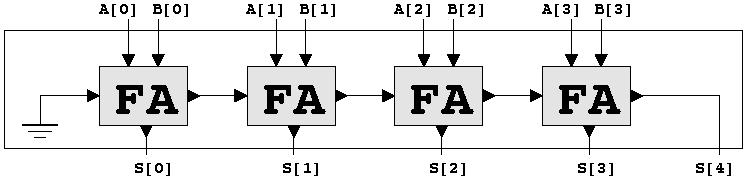
\includegraphics{adder.pdf}
  }
\caption{Addition of two integers (coded as bit vectors), using \emph{full adders.}\label{adder}}
\end{figure}

The following \alfa{} system describes a \emph{full adder}:
\index{full adder}
\begin{verbatim}
      system FullAdder (A,B,Cin : boolean) 
               returns (X,Cout : boolean);
      let
        X = A xor B xor Cin;
        Cout = (A and B) or (A and Cin) or (B and Cin);
      tel;
\end{verbatim}

To build an adder using this program, we need to 
instanciate a collection of such systems,
as shown in Fig.\ref{adder}. The shape of this collection may
be expressed as the {\alfa} domain \texttt{\{~b~|~0<=b<W~\}} where
\texttt{W} is a size parameter giving the number of bits of the
adder.
\index{use statement}
\index{use statement@\texttt{use}}

The \textbf{use} construct of {\alfa} allows precisely that. The
following system describes in {\alfa} the adder given in
Fig.~\ref{adder}:
\index{adder}
\index{binary addition}
\begin{verbatim}
system Plus: {W|W>1} (A,B: {b| 0<=b<W} of boolean)              -- 1       
             returns (S : {b| 0<=b<=W} of boolean);             -- 2       
var                                                             -- 3       
  Cin, Cout, X : {b| 0<=b<W} of boolean;                        -- 4       
let                                                             -- 5       
  Cin[b] =                                                      -- 6       
    case                                                        -- 7       
      {| b=0} : 0[];                                            -- 8       
      {| b>0} : Cout[b-1];                                      -- 9       
    esac;                                                       -- 10      
  use {b| 0<=b<W} FullAdder[] (A,B,Cin) returns(X, Cout);       -- 11      
  S[b] =                                                        -- 12      
    case                                                        -- 13      
      {| b<W} : X;                                              -- 14      
      {| b=W} : Cout[W-1];                                      -- 15      
    esac;                                                       -- 16      
tel;                                                            -- 17      
\end{verbatim}
In this system, line 11 reads as follows: 
\index{use statement}
\index{use statement@\texttt{use}}
\begin{quote}
"Use (or instantiate)
a collection of
instances of the subsystem \texttt{FullAdder}. This collection has the
shape of the extension domain\index{extension domain} 
\verb!{ b | 0<=b<W }! and is thus indexed
by index \texttt{b}. Let the inputs of the \texttt{b}-th instance be
the variables \texttt{A}, \texttt{B} and \texttt{Cin} at point
\texttt{b}, and similarly let the outputs of this collection of
instances be the variables \texttt{X} and \texttt{Cout}."
\end{quote}
Lines~6-10 describe the carry propagation, and lines~12-16
define the output of this binary adder.

\index{dimension extension}
In other words, line~11 is a shortcut for the following equations,
which are those of the system \texttt{FullAdder} whith the dimension
of the variables extended from zero to one:
\begin{verbatim}
        X[b] = A[b] xor B[b] xor Cin[b];
        Cout[b] = (A[b] and B[b]) or (A[b] and Cin[b]) or (B[b] and Cin[b]);
\end{verbatim}

\paragraph{Note.} In general, the extension indexes are 
added {\em to the left} of the existing indexes. This
cannot be seen in this example, since the full adder subsystem
has no indexes. 

\subsection{Handling structured programs}
A structured program is stored in {\mmalfa{}} as a {\mma{}} list of
systems called a \emph{library}. The default library is stored in the
global variable \verb!$library!.
\index{library}
\index{library@\texttt{\$library}}

A structured program may be written in one single file or several
distinct files.  In the former case the \texttt{load[]} function
returns a library composed of all the systems contained in the file,
and stores this library in \verb!$library!. %$ 
\index{load@\texttt{load}}

In addition, two functions, \texttt{putSystem[]} and
\texttt{getSystem[]}, may be used to get a system from a library
as the current system \texttt{\$result}\index{result@\texttt{\$result}}, and conversely
and to put back a modified system into a library. 
Typically a
system is extracted from the library as the {\em current}
system, modified by some program
transformation, and then put back in the library.
\index{putSystem@\texttt{putSystem[]}}
\index{getSystem@\texttt{getSystem[]}}

The commands to be used are \texttt{getSystem[]} and
\texttt{putSystem[]}.

\subsection{Program transformations associated with structures}

Most \mmalfa{} functions handle parameterized programs and \emph{use}
statements. There are, however, some major exceptions such as the
\texttt{cGen} translator\index{cGen@\texttt{cGen}} which generates code
only for {\em flat} {\Alpha} programs without subsystems. 
\mmalfa{}
provides functions to transform a structured program
into a flat equivalent one:
\begin{itemize}
\item \texttt{assignParameterValue[]}
\index{assignParameterValue@\texttt{assignParameterValue[]}}
gives a value to a size parameter, i.e. it refines a generic system
into a specialized one.
\item \texttt{inlineSubSystem[]}
\index{inlineSubSystem@\texttt{inlineSubSystem[]}}
expands a
\emph{use} statement, replacing it with the equations of the
corresponding subsystem, properly modified to take the dimension
extension into account.\index{flattening a structured program}
\item \texttt{inlineAll[]}
\index{inlining a subsystem}
\index{inlineAll@\texttt{inlineAll[]}}
recursively flattens a
structured {\alfa} program. \texttt{inlineAll[exceptions->\{sys\}]}
inlines all subsystems but those whose names appear in the 
exception list.
\end{itemize}

\paragraph*{More on subsystems}
For more information see 
{the subsystem documentation} in file
\begin{verbatim}
$MMALPHA/doc/Users/SubSystems.pdf
\end{verbatim}
If you are interested in scheduling structured subsystem, 
see an example in the \texttt{More} section of the 
\texttt{Master} notebook. 

\paragraph*{Troubleshouting}
There is a nasty bug in \texttt{inlineSubSystem} and
\texttt{inlineAll}. If you try to inline, with extension, 
a scalar equation, this equation must be given in 
standard notation, not in array notation. In Example~\ref{bug},
the equation in the called system must not be
written \texttt{out[] = 2[] + in[]}.
\begin{ex}{~}
\begin{verbatim}
system called (in: integer) returns (out: integer);
let
  -- This works
  out = 2.(->) + in;
tel;
system caller : {N | N>=1}
 (v: {i| 0< i <= N} of integer) 
 returns (w: {i| 0< i <= N} of integer);
let
  use {i| 0<i<=N} called (v) returns (w);
tel;
\end{verbatim}
\label{bug}
\end{ex}
\section{And now?}
\label{andnow}
In this document, we have presented a few possibilities of 
\mmalfa{}. You should now know if you are interested in 
using the \mmalfa{} software. 

If this is the case, you will find in the \alfa{} distribution 
some additional examples. See appendix~\ref{mmalphacontent}.

\bibliographystyle{alpha}
\bibliography{AlphaStart}

\newpage
\appendix
\section{Definition of \Alpha}
\label{alpha1}

\subsection{Meta Syntax}
\begin{tabbing}
xxxxxxx\= xxxxxxxxxxxxxxxxxx\= xxxxxxxxx\= xxxxxxx\= \kill
\>{\sl phrase* } \>===\>  zero or more repetitions of {\sl phrase}.\\
\> {\sl phrase1 {\sl \Alt} phrase2} \>===\> alternation, either {\sl
phrase1} or {\sl phrase2}.\\
\>  [\ldots] \>===\> optional phrase.\\
\> \Group{\ldots} \>===\> syntactic grouping.\\
\> {\bf \tt bold} \>===\> a terminal.\\
\> {\sl Italic} \>===\> a non-terminal.\\
\end{tabbing}

\subsection{Systems}
\Program{} stands for a library of \alfa{} programs. 
\PDecl{} (or \SystemDecl) is a single system. 
\Name{} is a system name. \ParamDecl{} is the declaration 
of a parameter domain. 
\InputDeclList{} is the list of input declarations. 
\OutputDeclList{} is the list of output declarations. 
\LocalDeclList{} is the list of local declarations. 
{\tt
\begin{tabbing}
xxxxxxxxxxxxxxxx\= xxx\= xx\=  xx\= \kill
\Program     \> :: \>\> \PDecl\ \PDecl *\\
\PDecl       \> :: \>\> \SystemDecl\\
\\\SystemDecl   \> :: \>\> system\ \Name \Opt{ : \ParamDecl }
                                    ( \InputDeclList )\\
\> \>\>\>  returns ( \OutputDeclList ) ;\\
\> \>\>\> \Opt{ var \LocalDeclList ;} \\
\> \>\>\> \EquationBlock ;\\
\\
\Name \>::\>\> \Identifier\\
\\
\ParamDecl  \> :: \>\> \Domain \\
\\
\InputDeclList \>::\>\> \VarDeclList\\
\OutputDeclList \>::\>\> \VarDeclList\\
\LocalDeclList \>::\>\> \VarDeclList\\
\end{tabbing}
}

\subsection{Declarations of variables}
\VarDeclList{} stands for a variable declaration. 
Notice that scalar types have been extended to 
special hardware types, such as 
\texttt{integer[S,10]} -- a signed
10 bit integer -- or
\texttt{integer[U,10]} -- an unsigned
10 bit integer. 
{\tt
\begin{tabbing}
xxxxxxxxxxxxxxxx\= xxx\= xx\=  xx\= \kill
\VarDeclList \>::\>\> \VarDeclaration *\\
\VarDeclaration \>::\>\> \IdentifierList\ : \Opt{\Domain of} \ScalarType ;\\
\ScalarType \> ::\>\> integer \Alt\ real \Alt\ boolean
\end{tabbing}
}

\subsection{Domains}
\Domain{} stands for a domain declaration. \IndexList{} is
a list of indexes, and \ConstraintList{} a list of constraints. 

Notice that operations on domains such as intersection
(\texttt{\&}), union (\texttt{|}), complement (\texttt{~}) and
preimage by an affine function are allowed. The parser 
does the corresponding operation. 

I am not sure that the \texttt{convex} syntax, nor the 
domain expressions fully work...

\ConstraintList{} is a list of constraints, each one being an
increasing constraint, a decreasing constraint, or an 
inequality.
{\tt
\begin{tabbing}
xxxxxxxxxxxxxxxx\= xxx\= xx\=  xx\= \kill
\Domain \>::\>\> \{ \IndexList \verb~|~ \ConstraintList \}\\
\>\>\Alt\> \Domain \verb~|~ \Domain\\
\>\>\Alt\> \Domain \verb~&~ \Domain\\
\>\>\Alt\> \Domain .\AffineFunction\\
\>\>\Alt\> \verb'~' \Domain\\
\>\>\Alt\> \Domain .convex\\
\>\>\Alt\> ( \Domain )\\
\\
\IndexList\>::\>\> \Opt{\IndexList ,} \Identifier\\
\\
\ConstraintList\>::\>\> \Opt{\ConstraintList ;} \Constraint\\
\Constraint \>::\>\> \IncreasingSeq \Alt\ \DecreasingSeq \Alt\ \EqualitySeq\\
\IncreasingSeq \>::\>\> \Group{ \IncreasingSeq \Alt\ \IndexExpList }
  \Group{ < \Alt\ <= } \IndexExpList\\
\DecreasingSeq \>::\>\> \Group{ \DecreasingSeq \Alt\ \IndexExpList }
  \Group{ > \Alt\ >= } \IndexExpList\\
\EqualitySeq\>::\>\> \Group{ \EqualitySeq \Alt\ \IndexExpList } = \IndexExpList
\end{tabbing}
}

\subsection{Equations}
\EquationBlock{} is the block of equation declarations. 
\Equation{} represents an equation, which can be either 
in array notation (when the lhs has the form \texttt{var[...]})
or in standard notation. An equation can also be a \texttt{use} statement.
\footnote{I am not sure of the syntax for the 
paramAssignation with the dot...}

{\tt
\begin{tabbing}
xxxxxxxxxxxxxxxx\= xxx\= xx\=  xx\= \kill
\EquationBlock \>::\>\> let \EquationList tel \\
\EquationList  \>::\>\> \Opt{ \EquationList } \Equation\\
\Equation\>::\>\> \Identifier [ \IndexList ] = \Expression ;\\
\>\> \Alt\ \> \Identifier = \Expression ;\\
\>\> \Alt\ \> use \Opt{ \ExtensionDomain} \Identifier
                                    \Opt{.\ParamAssignation} \\
\>\>\>\>( \InputList )\\
\>\>\>\> returns ( \IdentifierList ) ;\\
\\
\ParamAssignation \>::\>\> \AffineFunction \\
\\
\InputList \>::\>\> \Opt{ \InputList , } \Expression\\
\\
\ExtensionDomain \>::\>\> \Domain \\
\end{tabbing}
}

\subsection{Expressions}
Expressions can be case expressions, if statements\footnote{\alfa{}
conditional statements are strict, that is to say, both branches
are evaluated, and moreover, the domain of the statement is 
the intersection of that of the condition and of the 
expressions.}, restrictions, affine dependencies, binary operations, 
unary operations, and reductions\footnote{Reductions are allowed, 
but few transformations are currently available.}
{\tt
\begin{tabbing}
xxxxxxxxxxxxxxxx\= xxx\= xx\=  xx\= \kill
\Expression\>::\>\> case \ExpressionList esac \\
\>\> \Alt\ \> if \Expression then \Expression else \Expression\\
\>\> \Alt\ \> \Domain :\Expression\\
\>\> \Alt\ \> \Expression .\AffineFunction\\
\>\> \Alt\ \> \Expression [ \IndexExpList ] \\
\>\> \Alt\ \> \Expression \BinaryOp \Expression\\
\>\> \Alt\ \> \BinaryOp ( \Expression, \Expression ) \\
\>\> \Alt\ \> \UnaryOp \Expression\\
\>\> \Alt\ \> reduce ( \CommutativeOp, \AffineFunction, \Expression ) \\
\>\> \Alt\ \> ( \Expression ) \\
\>\> \Alt\ \> \Identifier\\
\>\> \Alt\ \> \Constant\\
\\
\ExpressionList \>::\>\> \Opt{ \ExpressionList  } \Expression ;\\
\\
\BinaryOp \>::\>\> \CommutativeOp \Alt\ \RelativeOp \Alt\ - \Alt\ div \Alt\ mod\\
\CommutativeOp \>::\>\> + \Alt\ * \Alt\ / \Alt\ and \Alt\ or \Alt\ xor \Alt\ min \Alt\ max\\
\RelativeOp \>::\>\> = \Alt\ <> \Alt\ < \Alt\ <= \Alt\ > \Alt\ >=\\
\UnaryOp \>::\>\> - \Alt\ not \Alt\ sqrt\\
\\
\Constant \>::\>\> \IntegerConstant \Alt\ \RealConstant \Alt\ \BooleanConstant\\
\end{tabbing}
}
\subsection{Dependance Functions and Index Expressions}
\AffineFunction{} stands for affine functions. 
{\tt
\begin{tabbing}
xxxxxxxxxxxxxxxx\= xxx\= xx\=  xx\= \kill
\AffineFunction \>::\>\> ( \IndexList -> \IndexExpList )\\
\IndexExpList \>::\>\> \Opt{ \IndexExpList, } \IndexExpression\
          \Alt\ \IndexExpression\\
\IndexExpression \>::\>\> \IndexExpression \Group{+ \Alt\  - } \IndexTerm\
          \Alt\ [ - ] \IndexTerm\\
\IndexTerm \>::\>\> \IntegerConstant \Identifier \Alt\ \IntegerConstant \Alt\ \Identifier
\end{tabbing}
}


\subsection{Terminals}
{\tt
\begin{tabbing}
xxxxxxxxxxxxxxxx\= xxx\= xx\=  xx\= \kill
\IntegerConstant \>::\>\> \Opt{-} \Number\\
\RealConstant \>::\>\> \Opt{-} \Number .\Number\\
\BooleanConstant \>::\>\> true \Alt\ false \Alt True \Alt\ False\\
\Number \>::\>\> \Digit \Digit *\\
\Digit \>::\>\> 0 \Alt\ 1 \Alt\ldots\Alt\ 9\\
\Identifier \>::\>\> \Letter \Group{\Letter \Alt\ \Digit} *\\
\Letter \>::\>\> a \Alt\ldots\Alt\ z  \Alt\ A \Alt\ldots\Alt\ Z \Alt\ \verb'_'\\
\end{tabbing}
}
Note: avoid using underscores...

\section{Description of the internal format of ASTs}
\label{ast}
This section describes the format of Abstract Syntax Trees (AST) of
\alfa{} programs, as handled by \mma{}. In other words, 
the AST of a program is the \mma{} expression that \MMAlfa{} stores in 
variable \texttt{\$result} when the \texttt{load} command is 
executed. It can be displayed just by having \mma{} evaluate
the expression \texttt{\$result}.

In the following description, non terminals are
written inside angle brackets \verb\<>\.  
For readability, keywords are
written without the prefix \texttt{Alpha`} which is implicit. 
For example, the keyword \texttt{system} is actually represented
by the symbol \texttt{Alpha`system}. 
The documentation is presented in
five sections: Systems, Domains, Equations, Matrices and General.

\subsection{Systems}
\begin{verbatim}
   <library>       ::= {<system> , ... , <system>} 
   <system>        ::= system [ <system_id>,
                                <param_space>, 
                                <in_var>, 
                                <out_var>,
                                <local_var>, 
                                <equation_list> ]
   <param_space>::= <domain>
   <in_var>     ::= <declare_list>
   <out_var>    ::= <declare_list>
   <local_var>  ::= <declare_list>
   <declare>    ::= decl [ <id>, <data_type>, <domain> ]
   <data_type>  ::= integer | boolean | real | notype
\end{verbatim}

\subsection{Domains}
The domain specification closely follows the internal format of the domain
definition in the domain library. This was done to minimize the overhead of
domain storage and of making library calls.  In Mathematica, domains should
only be changed by making calls to the domain library.

\begin{verbatim}
   <domain>     ::= domain [ <dimension_number>,
                             <id_list>, 
                             <polyhedron_list> ] 
   <polyhedron> ::= pol [ <constraints_number>, 
                          <rays_number>,
                          <equations_number>, 
                          <lines_number>,
                          <constraint_list>, 
                          <ray_list> ] 
   <constraint> ::= { <const_type>, 
                      <number>, ... , <number> }
   <const_type> ::= 0 | 1
                    0 / 1 = constraint is equality / inequality
   <ray>        ::= { <ray_type>, 
                      <number>, ... , <number> }
   <ray_type>   ::= 0 | 1
                    0 / 1 = ray is line / ray
\end{verbatim}

\subsection{Equations}
\begin{verbatim}
   <equation>   ::= equation [ <id>, <exp> ]
                  | use [ <id>, 
                          <extension>, 
                          <param_assign>, 
                          <exp_list>,
                          <id_list> ]
   <extension>  ::= <domain>
   <param_assign> ::= <matrix>

   <exp>        ::= var[<id>]
                  | const[<number>] | const[<boolean>] | const[<real>]
                  | binop [ <bop>, <exp>, <exp> ]
                  | unop  [ <uop>, <exp> ]
                  | if [ <exp>, <exp>, <exp> ]
                  | affine [ <exp>, <matrix> ]
                  | restrict [ <domain>, <exp> ]
                  | case [ <exp_list> ]
                  | call [ <id>, <exp_list> ]
                  | reduce [ <casop>, <matrix>, <exp> ]
   <bop>        ::= add | sub | mul | div | idiv | mod | min | max
                  | eq | le | lt | gt | ge | ne | or | and | xor
   <unop>       ::= neg | not | sqrt 
   <casop>      ::= add | mul | and | or | xor | min | max
\end{verbatim}

\subsection{Matrices}
\begin{verbatim}
   <matrix>     ::= matrix [ <rows_number>,
                             <cols_number>, 
                             <id_list>, 
                             { { <number>, <number>, ... , <number> },
                               { <number>, <number>, ... , <number> },
                               ...
                               { <number>, <number>, ... , <number> } } ]
\end{verbatim}

\subsection{General specifications}
Numbers, ids, and lists, as used above, are defined generally
(with \verb\<*>\ representing any nonterminal ).

\begin{verbatim}
   <*_number>   ::= <number>
   <*_id>       ::= <id>
   <*_list>     ::= { <*>, <*>, ... , <*> }

   <number>     ::= [0-9][0-9]* | Infinity
   <real>       :=  <number>.<number>
   <boolean>    ::= True | False
   <id>         ::= "a name"
   <comment>    ::= (* blah blah blah *)
\end{verbatim}

\texttt{Reserved Keywords}

\begin{verbatim}
        Alpha`add       Alpha`affine    Alpha`and       Alpha`binop
        Alpha`boolean   Alpha`call      Alpha`case      Alpha`const
        Alpha`decl      Alpha`div       Alpha`domain    Alpha`eq
        Alpha`equation  Alpha`ge        Alpha`gt        Alpha`idiv
        Alpha`if        Alpha`integer   Alpha`le        Alpha`lt
        Alpha`matrix    Alpha`max       Alpha`min       Alpha`mod
        Alpha`mul       Alpha`ne        Alpha`neg       Alpha`not
        Alpha`notype    Alpha`or        Alpha`pol       Alpha`real
        Alpha`reduce    Alpha`restrict  Alpha`sqrt      Alpha`sub
        Alpha`system    Alpha`unknown   Alpha`unop      Alpha`use
        Alpha`var       Alpha`xor
\end{verbatim}

\section{A brief description of the \MMAlfa{} distribution}
\label{mmalphacontent}

\subsection{The \texttt{Master} notebook}
The master notebook is open by the \texttt{start[]} 
command. It contains 6 sections.
\begin{itemize}
\item The welcome section. 
\item The introduction notebooks: the 
\texttt{getting-started}\index{getting-started@The \texttt{Getting-started} notebook}
notebook, and the \texttt{mma-intro}\index{mma-intro@The \texttt{mma-intro} notebook}
notebook. 
\item The simple examples section. It contains pointers to the 
matrix-vector, the Fir filter, the Fifo, and the delay line 
demonstrations. 
\item The advances examples section. Here are presented a demonstration
of the Delayed Least-Mean Square filter, of the structured scheduler, 
and of the Samba architecture for DNA sequence alignment.
\footnote{Do the DLMS... Check the structured scheduler...}
\item More contains an access to the Domlib notebook, and some
suggestion about the organization of your own notebooks. It 
explained how you can set the variables \texttt{\$myNotebooks},
\texttt{\$myMasterNotebook}, then use the \texttt{myStart[]} 
and the \texttt{link}
commands to access directly your own working space. 
\item Finally, the Tests section gives access to a test notebook. 
\end{itemize}

\subsection{Documentation}
To explore the \MMAlfa{} distribution, you can follow the 
html files which are in each subdirectory of the distribution.
The structure of 
the distribution is as follows. The main directory is called \MMAlfa{}. It
contains another directory called Mathematica which is the 
\MMAlfa{} distribution properly speaking. In the \MMAlfa{} directory, 
the file \texttt{welcome.html} gives access to the documentation. 

The Mathematica directory is organized as follows:
\begin{itemize}
\item \texttt{bin.cygwin} and \texttt{bin.solaris} 
directories contain the binary files for execution of \MMAlfa{} on 
the Windows NT and Solaris system respectively. 
\item \texttt{config} contains the configuration files.
\item \texttt{demos} contains the demonstrations notebooks.
\item \texttt{doc} contains the documentation notebooks.
\item \texttt{lib} contains the Mathematica packages which form 
\MMAlfa{}.
\item \texttt{sources} contains the source files of the \C{} programs
and of the latex documentation files. 
\item \texttt{tests} containes the test programs for \MMAlfa{}.
\end{itemize}

\printindex

\newpage
\tableofcontents


\end{document}